\section{Parceive}
\label{sec:parceive}
We implemented Parceive, a tracing-based tool for interactive software
analysis. Its vision is to aid developers with identifying parallelism
opportunities on various granularity levels. Parceive utilizes static binary
analysis and dynamic instrumentation to collect trace data. Being less
conservative than purely static approaches let us focus on concurrency-related
events, e.g., memory accesses, routine invocations, and object instantiations.
By a-posteriori abstraction of such fine-grained information we infer
architectural aspects of user applications. Here is the difference to most
existing tools, the results may be used as a starting point for an extensive
architecture refactoring. However, the user is responsible for a correct
parallelization due to the inherent incompleteness of dynamic analysis.

\begin{figure}[h!]
	\begin{center}
		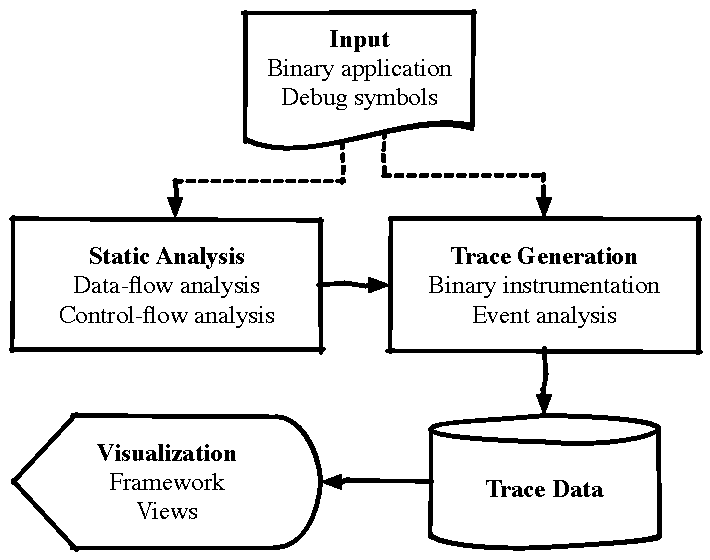
\includegraphics[width=0.40\textwidth]{img/parceive}
		\caption{Components of Parceive}
		\label{fig:parceive_overview}
	\end{center}
\end{figure}

Figure \ref{fig:parceive_overview} depicts the fundamental components of
Parceive and its relations. Several analyses operate on user applications in
binary form to generate trace data. These analyses can be classified into
static analyses and runtime analyses. The former inspect the data- and
control-flow of single linkage objects. By incorporating given symbol
information, static analyses enable our tool to infer global properties, e.g.,
stack variables and their accesses, loop constructs, or class hierarchies.
Additionally, the gathered knowledge is used to tailor the scope of the
subsequent runtime analyses to reduce overhead.

These runtime analyses instrument and inspect predefined events during actual
executions of the user applications, e.g., object instantiations, method
invocations, or thread handling (in case of multi-threaded user applications).
During such events Parceive collects trace data and efficiently writes it into
an SQLite database. The underlying database scheme enables highly specific and
performant queries for visualizations. The visualization component is the key
to comprehend and parallelize user applications. It lets user grasp complex
system behaviour by providing views for multiple viewpoints. It consists of a
visualization framework and several views that are based on the framework. Each
view simplifies and highlights specific aspects of the traced software. We
elaborate this in more detail in the next section.